\documentclass[a4paper,10pt]{article}

\usepackage[utf8x]{inputenc}

\usepackage[margin=1.2in]{geometry}
\usepackage{parskip}

\usepackage{amsmath}
\usepackage{amssymb}

\usepackage{graphicx}
\usepackage{float}

\usepackage{listings}
\usepackage[dvipsnames]{xcolor}
\definecolor{lightgray}{gray}{0.97}

\lstset{  
    backgroundcolor=\color{lightgray},   
    commentstyle=\color{gray},
    keywordstyle=\color{magenta},
    numberstyle=\tiny\color{cyan},
    stringstyle=\color{OliveGreen},
    frame=top,frame=bottom,
    basicstyle=\small\normalfont\sffamily,
    stepnumber=1,
    numbersep=10pt,
    tabsize=4,
    extendedchars=true,
    breaklines=true,
    captionpos=t,
    mathescape=true,
    showspaces=false,
    showtabs=false,
    xleftmargin=17pt,
    framexleftmargin=17pt,
    framexrightmargin=17pt,
    framexbottommargin=5pt,
    framextopmargin=5pt,
    showstringspaces=false
}


\title{Numerical Recipes in Astrophysics \\
        \large Assignment 1}
\author{Brendon Walter (s2078864)}


\begin{document}

    \maketitle

    \begin{abstract}
        In this first assignment for Numerical Recipes in Astrophysics (taught by Dr. Marcel van Daalen at Leiden University, Spring 2019), we use the algorithms learned in the first half of the course to ....
    \end{abstract}

    \tableofcontents

    \newpage
\section{Routines}

I created a file called \texttt{routines.py} which contains various functions that are used throughout this exercise. The full output is seen in Appendix \ref{sec:routines}.

The entire assignment is run through the script \texttt{handin1.py}. The relevant parts are shown in snippets throughout the rest of the file.


\lstinputlisting[language=Python, caption=\texttt{handin1.py} : header,
                 firstline=1, lastline=19]{handin1.py} \label{list:header}

    \newpage
    \subsection{Poisson Distribution}

    This function implements the Poisson distribution, defined as

    \begin{equation}
        P(k) = \frac{\mu^k e^{-\mu}}{k!}
        \label{eq:poisson}
    \end{equation}

    \lstinputlisting[language=Python, caption=\texttt{poisson.py}]{nur/poisson.py}
    \lstinputlisting[language=Python, caption=\texttt{handin1.py} : 1a,
                     firstline=30, lastline=36]{handin1.py}
    \lstinputlisting[language=Python]{output/1a_poisson.txt}



    \newpage
    \subsection{Random Number Generator}

    Here, I create a random number generator that uses a mix of multiplicative linear congruential generation:
    \begin{equation}
        x_{j+1} = a x_{j} + c \mod m
        \label{eq:mlcg}
    \end{equation}

    and a 64-bit XOR-shift:
    \begin{equation}
        \begin{array}{l}
        x_{j+1} = x_{j} \land (x_{j} \ll a) \\
        x_{j+1} = x_{j} \land (x_{j} \gg b) \\
        x_{j+1} = x_{j} \land (x_{j} \ll c)
        \end{array}
        \label{eq:xor_shift}
    \end{equation}

    I use the suggested values for the multipliers from the textbook.

    When called with \texttt{RNG.rand()}, the generator generates a number between 0 and 1. An additional function, \texttt{RNG.rand\_range()} allows the user to generate a float between two values.

    Typically usage of the generate uses the current Unix time in seconds as the starting seed. This ensures that it is as random as possible on start. For the purpose of this assignment, where I want the output to be reproducible, I assign a starting seed (see \ref{list:header}).

    In order to ensure that the same generator is used throughout the assignment, I create a singleton class from which the RNG inherits. 

    Figure \ref{fig:rng} below shows the output of the first 1,000 and 1,000,000 randomly generated numbers. It seems to perform well.

    \lstinputlisting[language=Python, caption=\texttt{RNG.py}]{nur/RNG.py}

    \newpage
    \lstinputlisting[language=Python, caption=\texttt{handin1.py} : 1b,
                     firstline=50, lastline=64]{handin1.py}
    
    \begin{figure}[H]
        \centering
        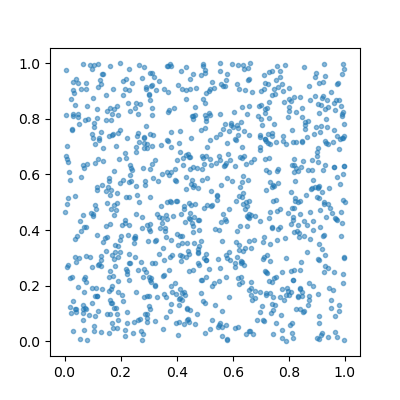
\includegraphics[height=6cm]{output/1b_RNG-scatter.png}
        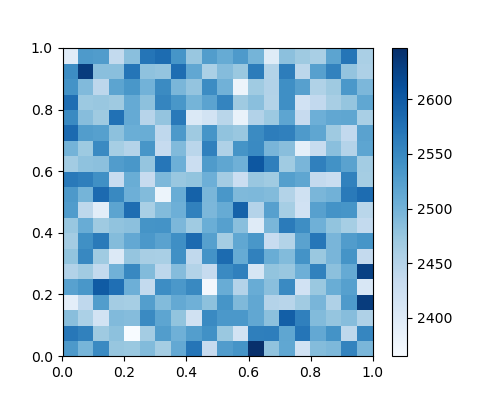
\includegraphics[height=6cm]{output/1b_RNG-hist2d.png}
        \caption{The first thousand (left) and million (right) pseudo random numbers from the above generator. The coordinates of each point are given as  ($x_j$, $x_{j+1}$)}
        \label{fig:rng}
    \end{figure}


    \newpage
\appendix
\section{\texttt{routines.py}} 
\label{sec:routines}

\lstinputlisting[language=Python, caption=\texttt{routines.py}]{nur/routines.py}


\newpage
\section{\texttt{integration.py}} 
\label{sec:integration}

\lstinputlisting[language=Python, caption=\texttt{integration.py}]{nur/integration.py}


\newpage
\section{\texttt{derivation.py}} 
\label{sec:derivation}

\lstinputlisting[language=Python, caption=\texttt{derivation.py}]{nur/derivation.py}


\newpage
\section{\texttt{interpolation.py}} 
\label{sec:interpolation}

\lstinputlisting[language=Python, caption=\texttt{interpolation.py}]{nur/interpolation.py}



\newpage
\section{\texttt{sampling.py}} 
\label{sec:sampling}

\lstinputlisting[language=Python, caption=\texttt{sampling.py}]{nur/sampling.py}



\newpage
\section{\texttt{galaxies.csv}} 
\label{sec:gal_gen}

\lstinputlisting[caption=\texttt{galaxies.csv}]{output/2d_galaxies.csv}



\newpage
\section{\texttt{sorting.py}} 
\label{sec:sorting}

\lstinputlisting[language=Python, caption=\texttt{sorting.py}]{nur/sorting.py}





\end{document}
